This section is devoted to provide a detailed description of the included video \footnote{Alternatively, the video can be consulted in this link \url{https://www.youtube.com/watch?v=ElxK_95n4lE&feature=youtu.be}}.
%
Specifically, to have a better understanding of the behaviour of each algorithm with the WFG5 problem a simulation is recorded.
%
The WFG5 problem is selected given its properties being perhaps the most difficult one --under standard parameterization-- of the WFG problems.
%
The main peculiarity of this problem dwell in its desceptiveness, which involves several local optimal regions that mislead the search process of the algorithms.
%
Principally, the Pareto geometry of this problem is convex, and such Pareto optimal solutions of the distance parameters have the following values:
%
\begin{equation}
   x_{i=k+1:n} = 2i \times 0.35
\end{equation}
Therefore, in this simulation is taken into account the standard parameterization indicated in the main document, as well the specified configuration.
%
Each algorithm was run with two objectives and two decision variables, whose number of position and distance parameters was set to one, and the number of generations was set to $1000$.
%

The video is vertically divided in two sides, the left-side and right-side representing each one the objective space and the decision variable space respectively.
%
In the decision variable space (right-side) each local optimal region is remarked by a horizontal blue line, and the global optimal region is remarked with a horizontal red line.
%
In this configuration, the position and distance parameters are denoted by $x_1$ and $x_2$ respectively.
%
The video shows that after ten generations the state-of-the-art-MOEAs have converged prematurely to the local optimal regions, contrarely to the VSD-MOEA which is still exploring.
%
Approximatelly on the $30\%$ of total generations, VSD-MOEA has located three individuals in the global optimal region, and in few generations later ($40\%$) has located several individuals around the optimal region.
%
At the $50\%$ of total generations, VSD-MOEA has converged to the optimal region (red horizontal line) avoiding the remaining sub-optimals (blue horizontal lines).
%
Finally, the remaining $50\%$ of generations VSD-MOEA keeps improving quality in the objective space.

%%Figures ONE TWO THREE, are taken of the video and belong to the 0\%, 50\% and 100\% of total generations.
%%
%%\begin{figure}[t]
%%\centering
%%\begin{tabular}{l}
%% 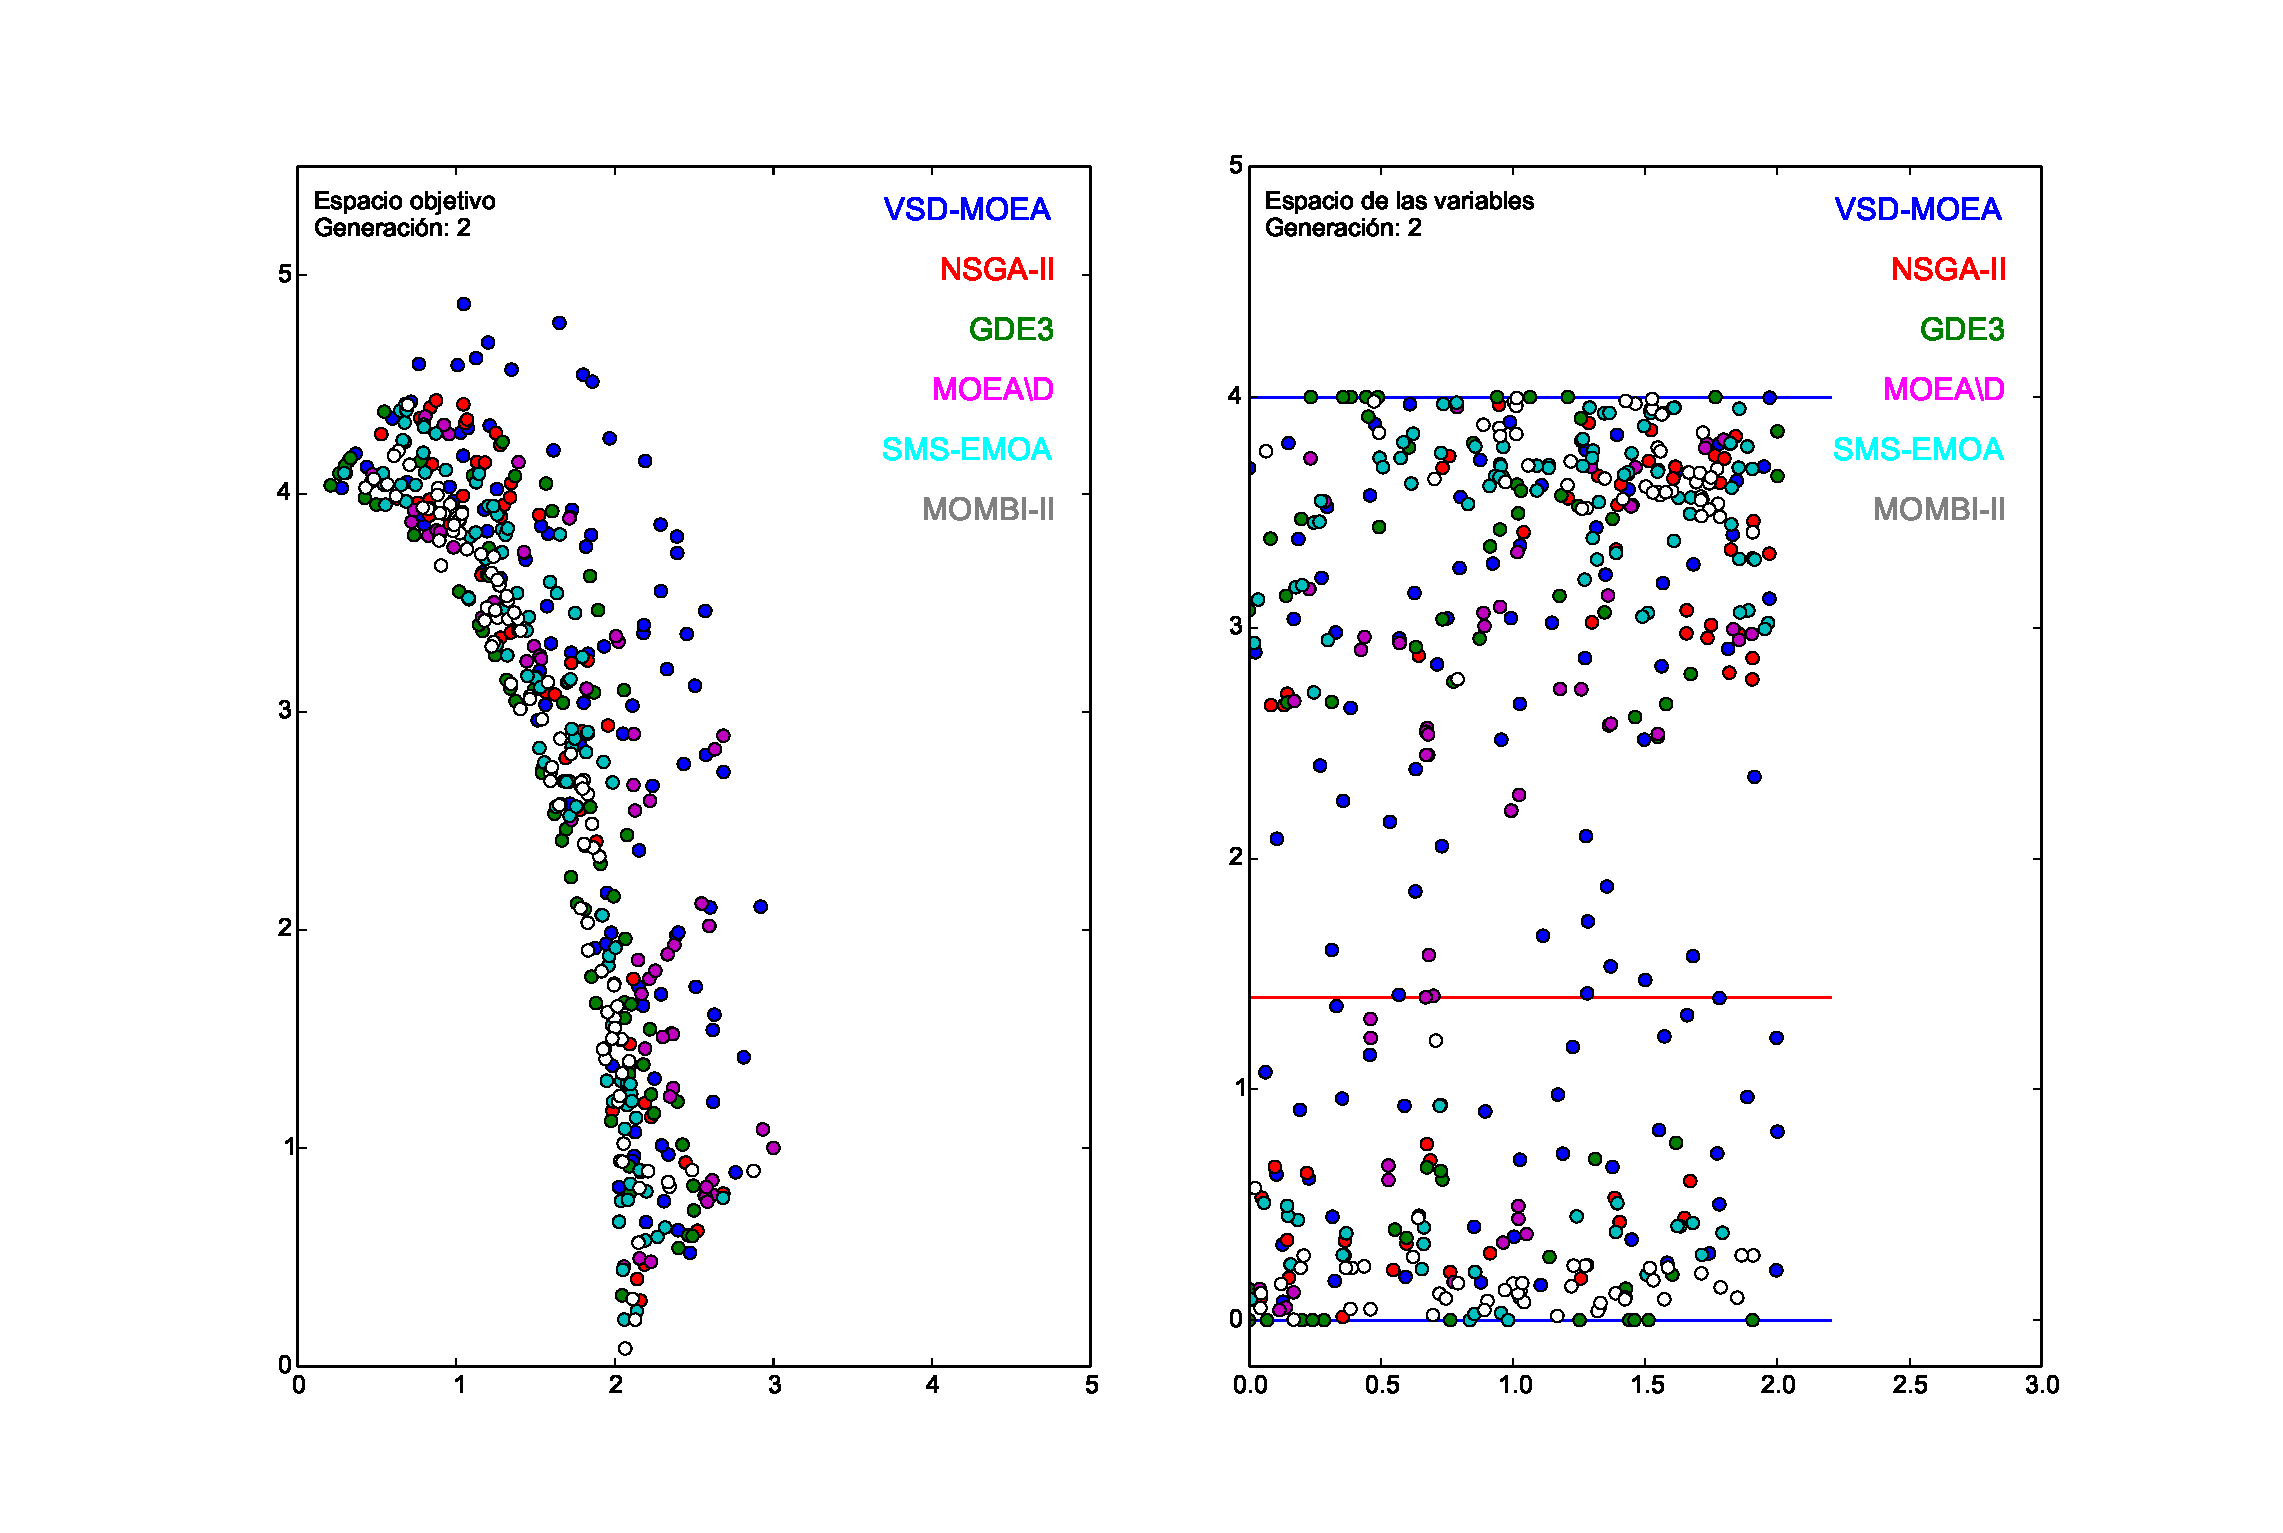
\includegraphics[scale=0.3]{Images/Simulacion_Algoritmo_1.eps}\\[0cm]%[-0.14cm] 
%% 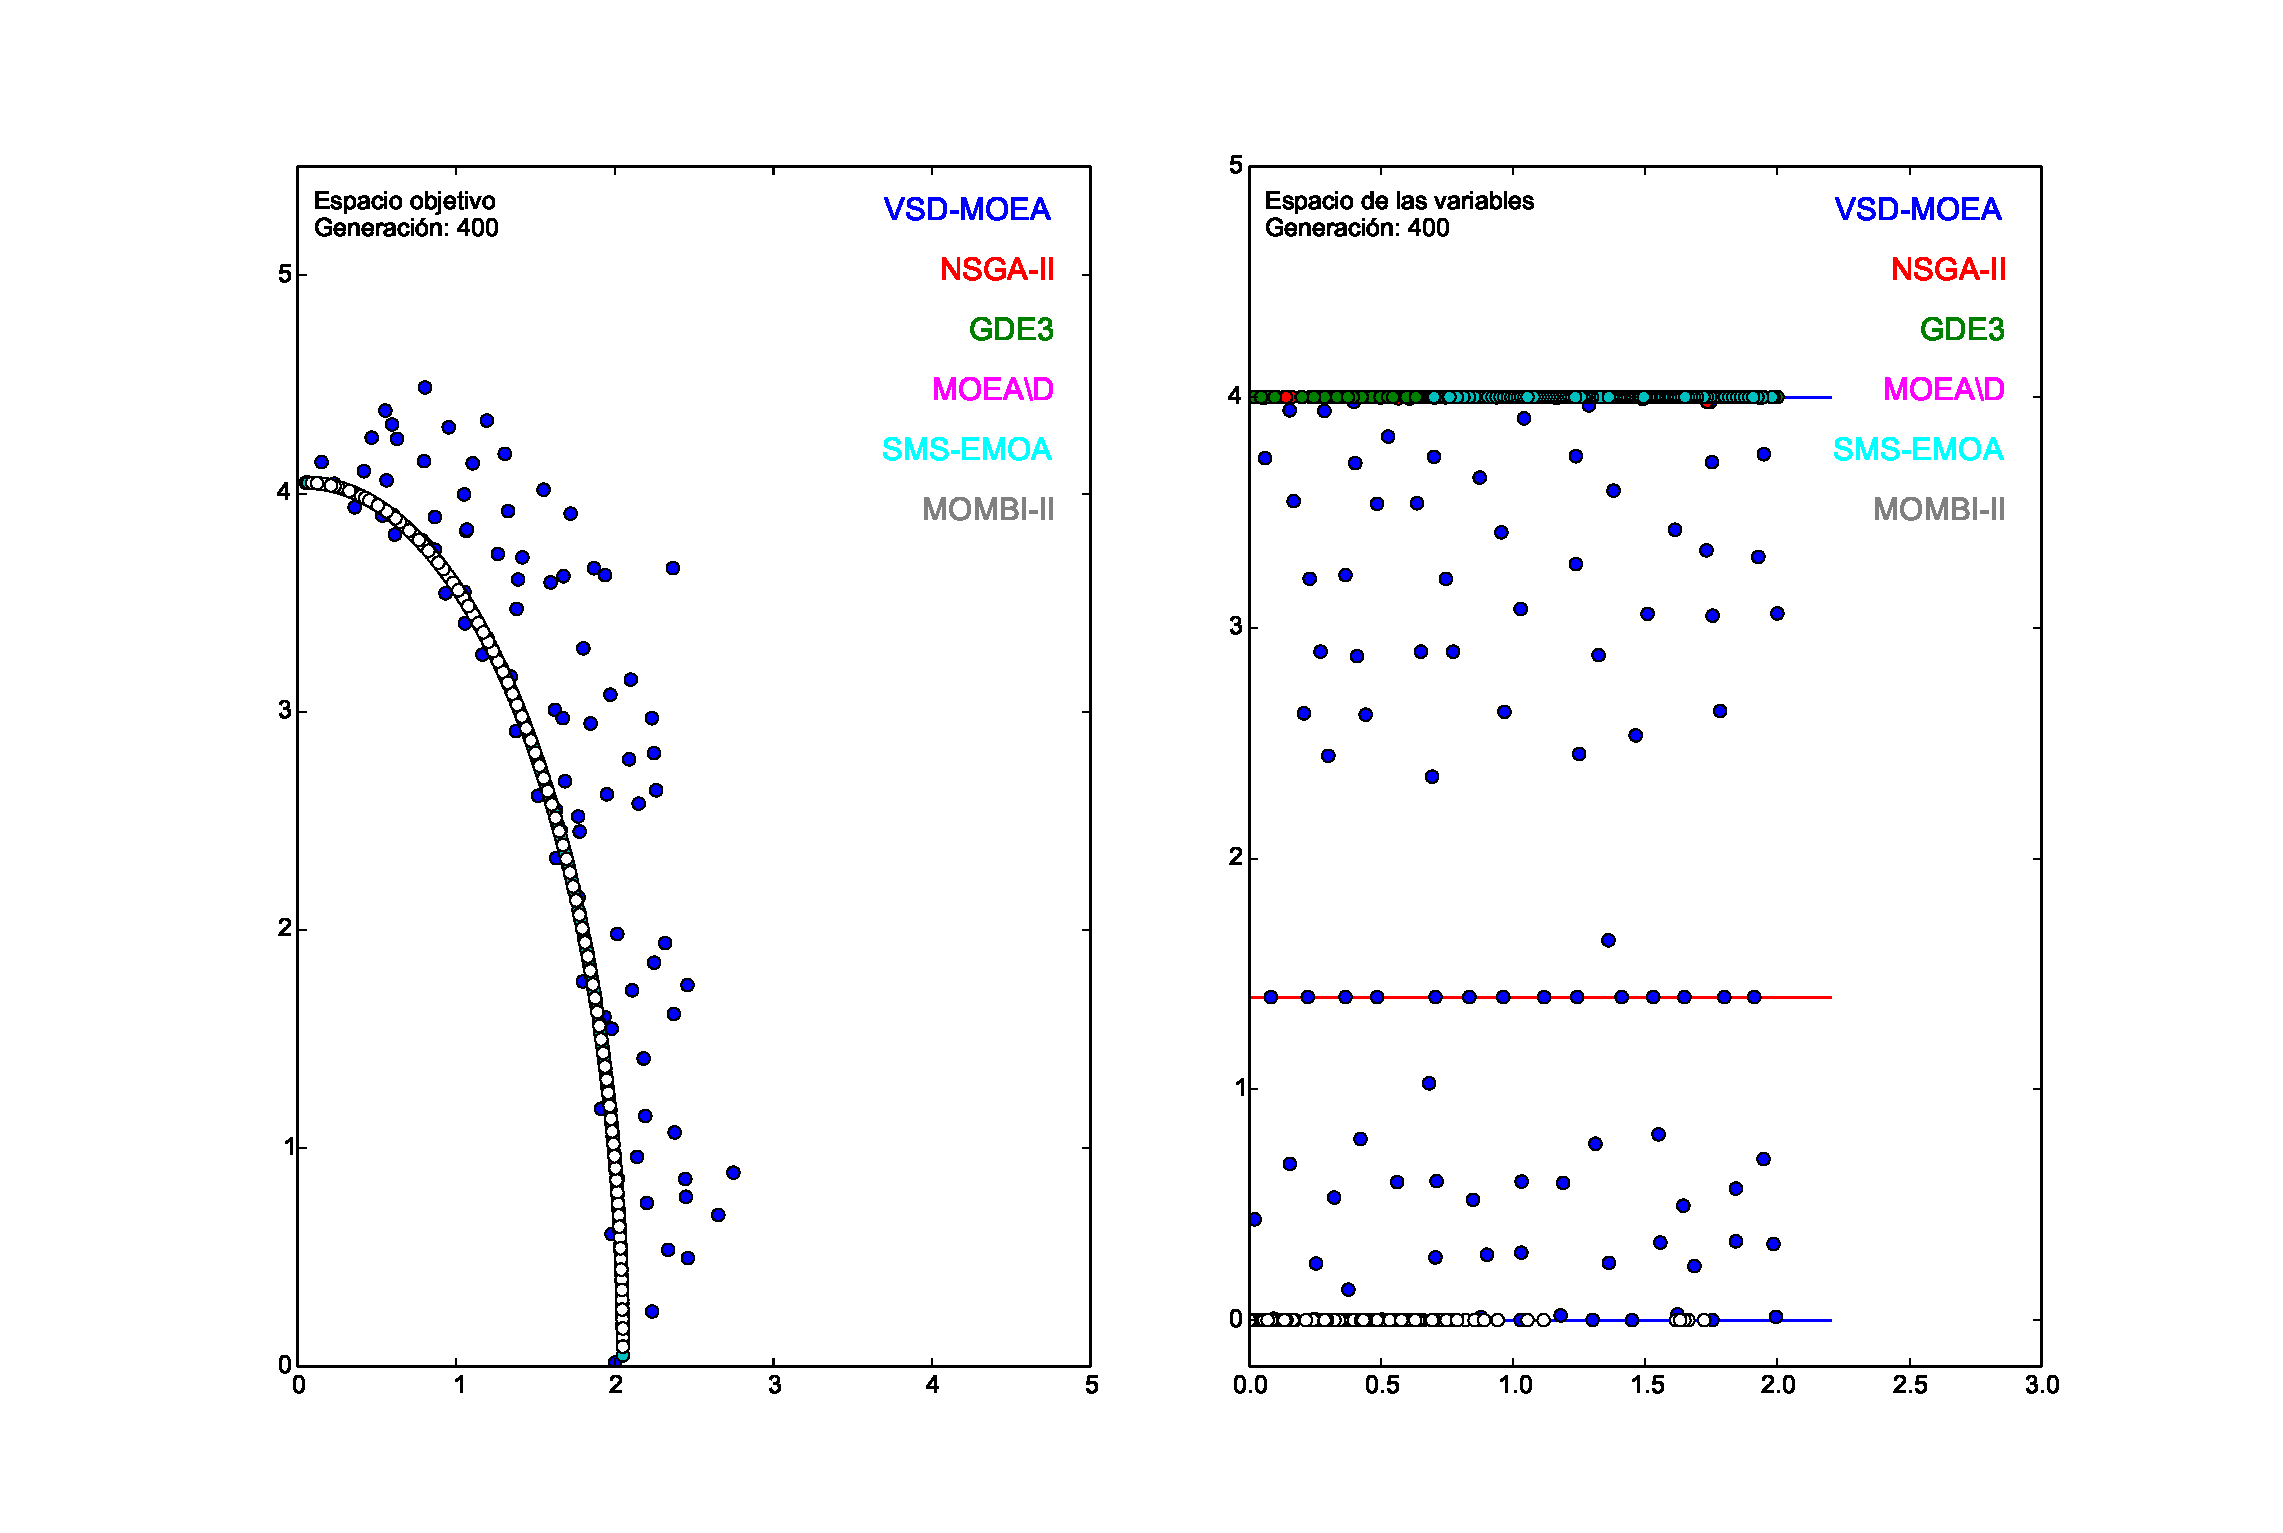
\includegraphics[scale=0.3]{Images/Simulacion_Algoritmo_4.eps}\\[0cm]%[-0.14cm] 
%% 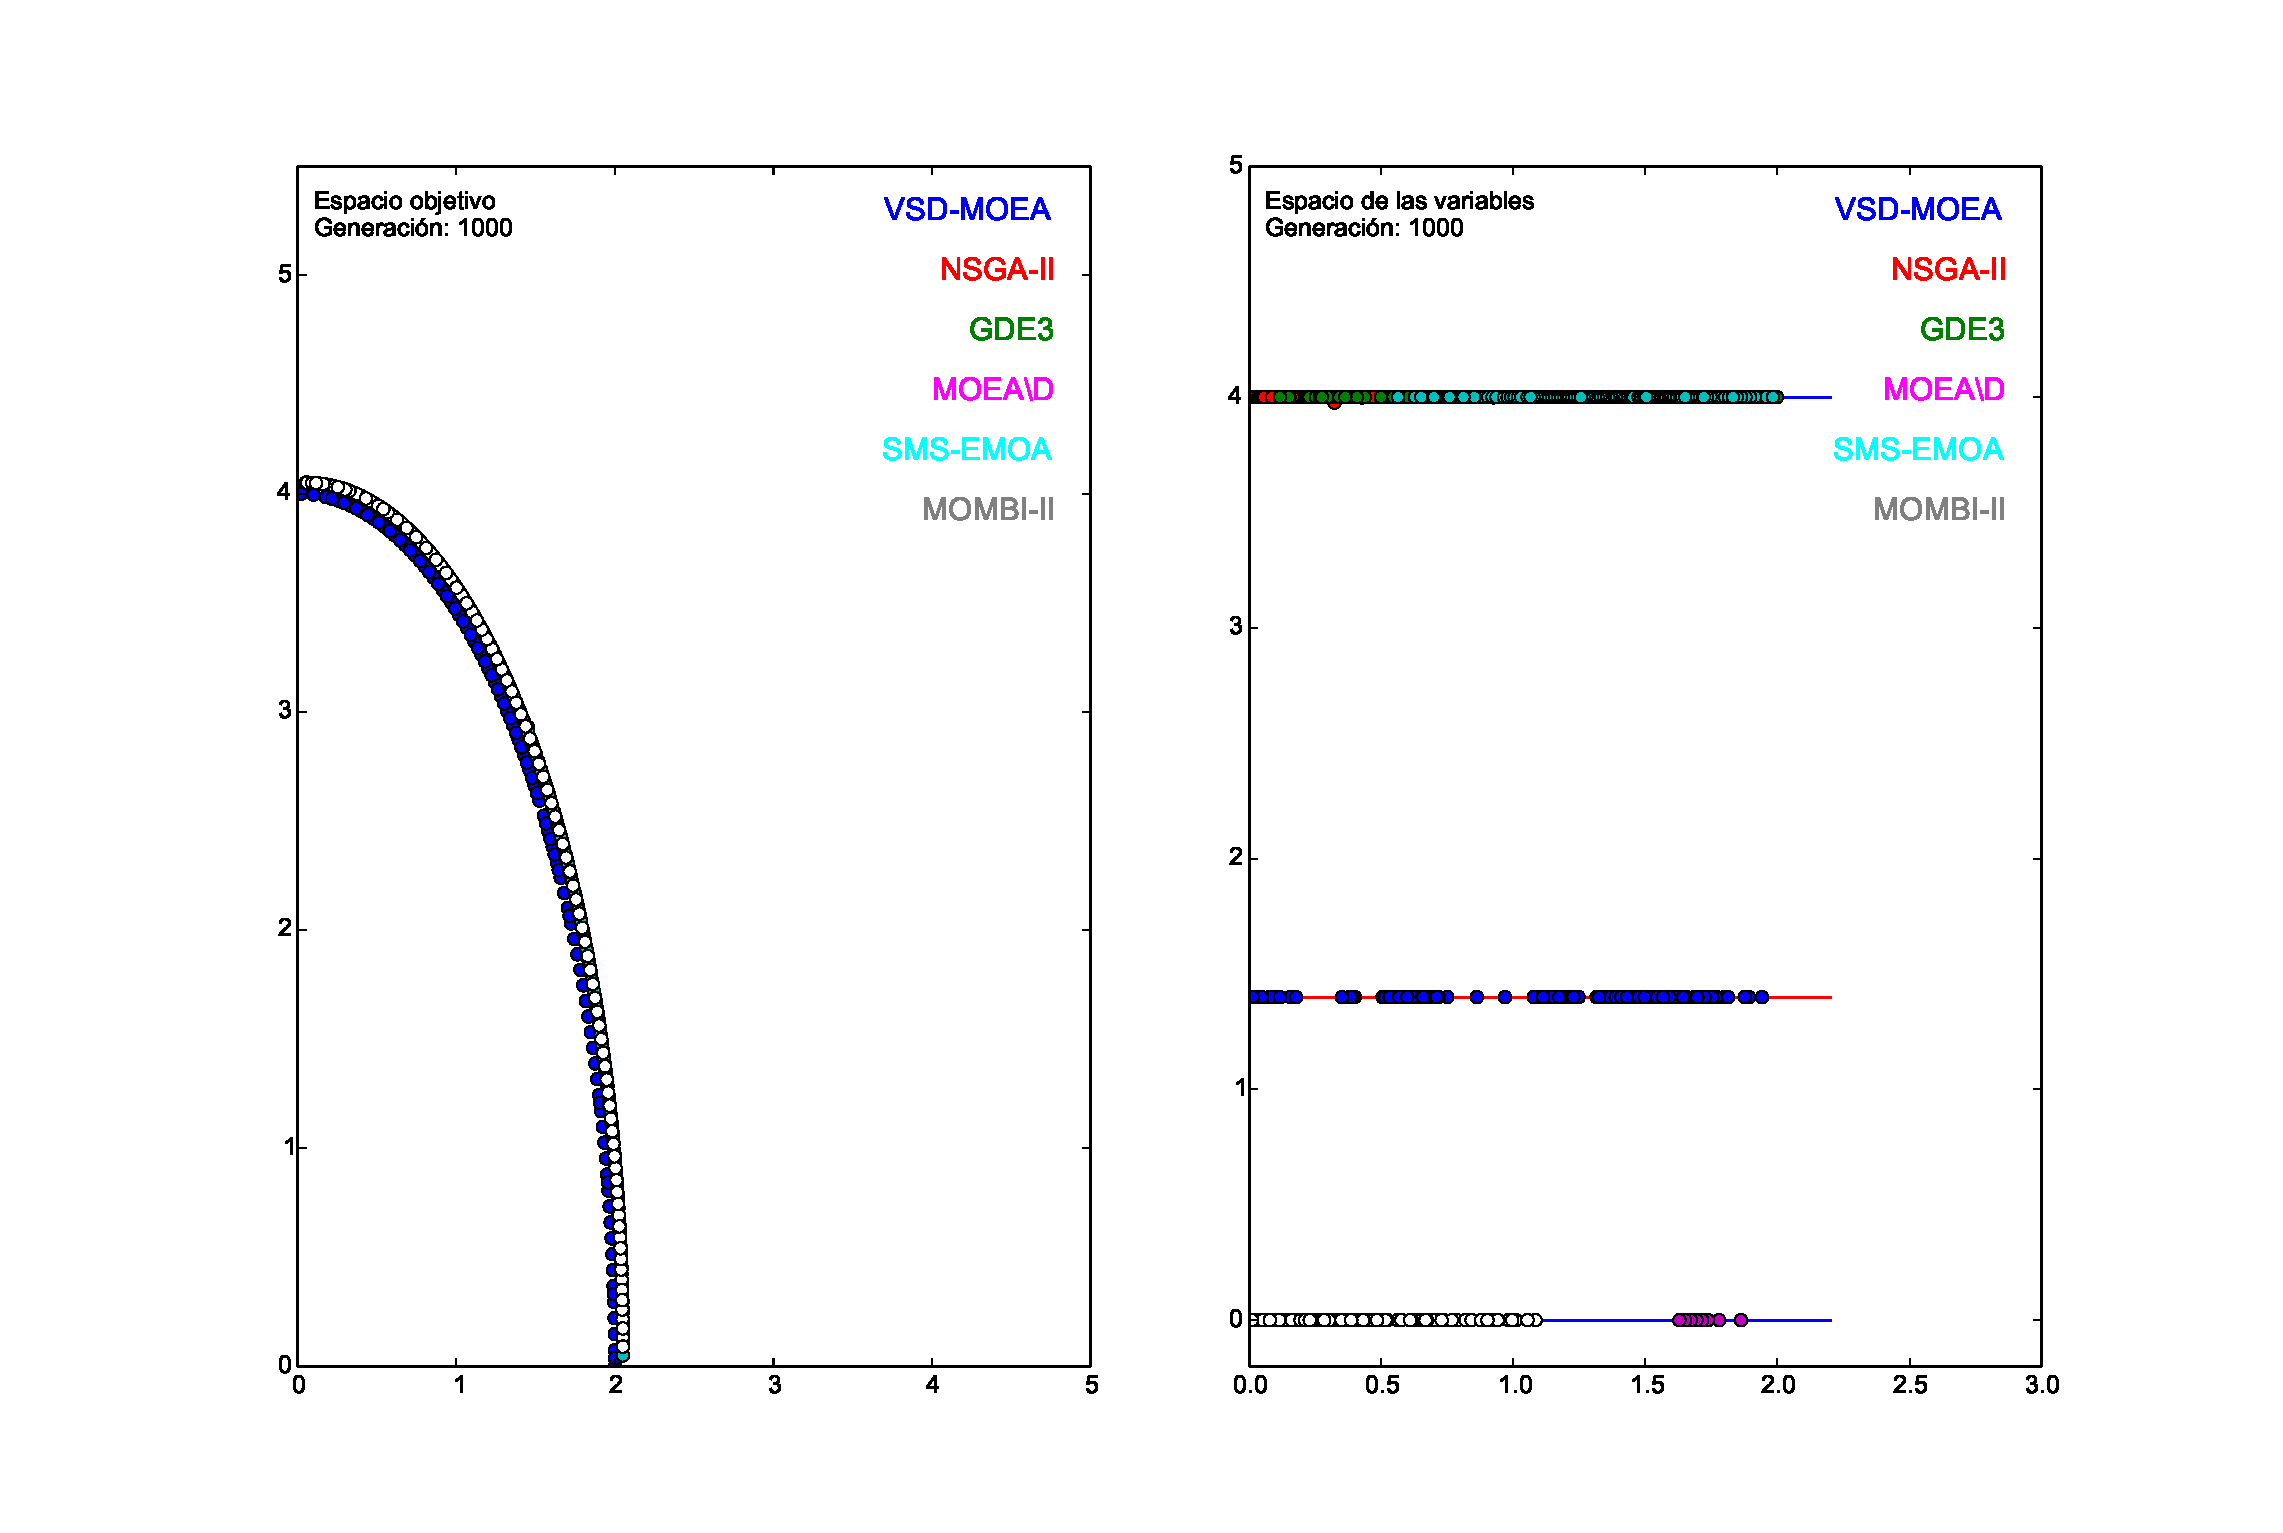
\includegraphics[scale=0.3]{Images/Simulacion_Algoritmo_5.eps}\\[0cm]%[-0.14cm] 
%%\end{tabular}
%%\caption{Performance of \MOEAS{} for the problems with three objectives considering three ranges of stopping criterion: short-term (first row), middle-term (second row) and long-term (third row).}\label{fig:Performance_time_3obj}
%%\end{figure}
